\documentclass{article}

\usepackage{tikz}
 
\begin{document}

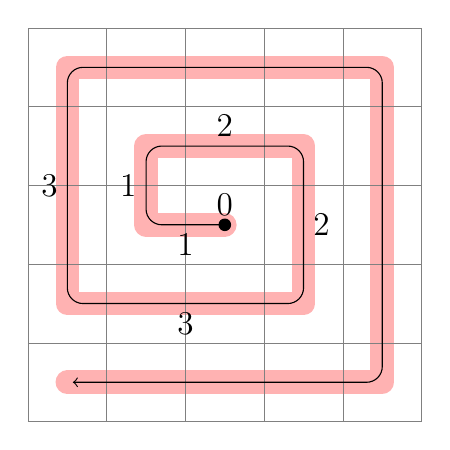
\begin{tikzpicture}
	\draw[line width=0.3cm,color=red!30,cap=round,join=round] 
		(2.5, 2.5) -- ++(-1, 0) -- ++(0, 1) -- ++(2, 0) -- ++(0, -2) -- ++(-3, 0) -- ++(0, 3) -- ++(4, 0) -- ++(0, -4) -- ++(-4, 0);
		
	\draw[help lines] (0, 0) grid (5, 5);
	\draw[above] (2.5, 2.5) node(s){\large $0$};
	\draw[below] (2,2. 5) node(s){\large $1$};
	\draw[left] (1.5, 3) node(s){\large $1$};

	\draw[above] (2.5, 3.5) node(s){\large $2$};
	\draw[right] (3.5, 2.5) node(s){\large $2$};

	\draw[below] (2, 1.5) node(s){\large $3$};
	\draw[left] (0.5, 3) node(s){\large $3$};

	\fill (2.5,2.5) circle (0.08cm);
	
  	\draw[->,rounded corners=0.2cm,shorten >=2pt]
		(2.5, 2.5) -- ++(-1, 0) -- ++(0, 1) -- ++(2, 0) -- ++(0, -2) -- ++(-3, 0) -- ++(0, 3) -- ++(4, 0) -- ++(0, -4) -- ++ (-4, 0);
\end{tikzpicture}

\end{document}
